Embedded programming has always been about dealing with the real world in a timely manner.

When you push a button on your microwave, it beeps and updates the display immediately. It doesn't matter if the microwave is currently making popcorn or not---it responds in near real-time to your touch. If you've ever tried to achieve this with your Arduino (or other embedded controller), you discovered that it is very difficult to make your embedded project do two things at once---like controlling a motor while waiting for a button to be pressed. You either found yourself writing large, complex loops that constantly check everything about your system, or you found yourself reading about ``interrupt vectors,'' and wondered if you should have paid more attention in your high school physics class.

\plumbing, and the language it is written in (\occam), makes these problems go away.

\newpage

\section*{Parallelism Yesterday}
%The Transputer was a processor ahead of its time.
\begin{floatingfigure}[r]{0.4\linewidth}
	  \begin{center}
    	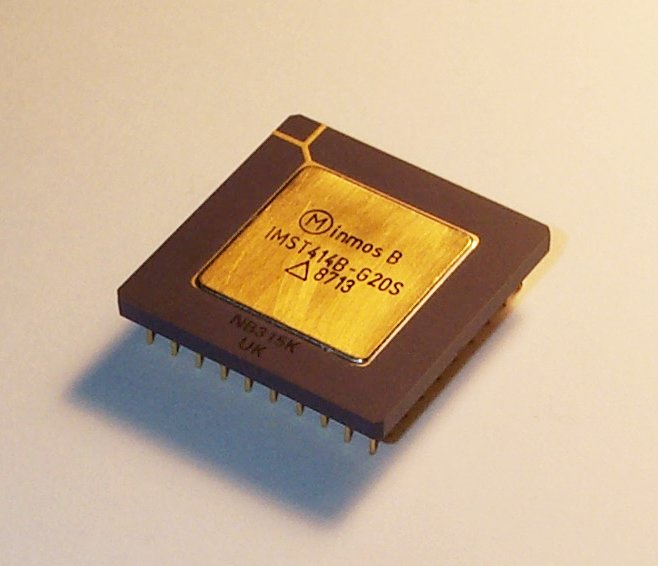
\includegraphics[width=0.4\linewidth]{images/t414}
			\captionsetup{labelformat=empty,justification=centering}
   		\caption{The T414.}
    	\label{image:t414}
  \end{center}
\end{floatingfigure}


\justoccam is an old programming language; it was developed in the early 1980's for use on the Transputer, a specialized processor developed by the British company inmos. This processor was special because it was able to switch between many thousands of parallel processes very, very quickly. It also had four special ``links'' that allowed it to be connected to other Transputers, instantaneously creating a distributed cluster of processors. \justoccam made it possible, in just a few lines of code, to write programs that would run across many processors in parallel, taking advantage of these networked clusters of Transputers.

In 2010, this may not seem impressive: for example, every computer shipped by Apple has at least two cores, as is the case with many computer manufacturers today. However, we are talking about {\strong parallel processors designed and manufactured nearly 30 years ago}. And the language, \justoccam, has evolved---it is now called \occam, and we have worked hard to make sure it runs on everything from your Arduino to your desktop computer, regardless of the operating system (Linux, Mac, Windows) you choose to use.

\newpage

\section*{Parallelism Today}
Thinking about handling things ``in parallel'' means handling them ``at the same time.'' With only one processor, you can only pretend to handle two things at once---we call this {\strong concurrency}. If you want to control a motor while waiting for a button to be pressed, or to control 64 LEDs ``at the same time,'' you could do it with a loop. The loop would get complex, and you'd be responsible for managing all of the concurrency in your code.

Or, you could use \occam. And on the Arduino, you could use our library of code, called \plumbing, to make these tasks much easier. For example, take a look at the code from Chapter~\ref{ch3}:~\nameref{ch3}. 

\vspace{3mm}
	\begin{lstlisting}[firstnumber=1]
PAR
  blink (11, 500)
  blink (12, 500)
	\end{lstlisting}

With the right circuit, this code would tell our Arduino to blink two LEDs in \PARallel, one on pin 11, and one on pin 12. The {\code blink} command comes from the \plumbing library of code, and the \PAR comes from \occam. Combined, the language and the library of code make it easy to express ideas about problems that involve two things happening ``at the same time,'' or (as we prefer to say), {\em concurrently}.

We assume that you, the reader, have little or no programming experience, but are excited to explore our tools with your trusty Arduino in hand. Please---enjoy.

\newpage

\section*{The Commons}

This text, as well as all of the tools you need to explore it, are free and open. Our text is made available under a Creative Commons license, our software under the LGPL, and we have chosen the Arduino (and its many variants) because of the open nature of that community as well. We encourage you to begin exploring parallel programming using \plumbing, \occam, and your Arduino. 

\ \\

\begin{figure}[ht]
	\begin{center}$
		\begin{array}{ccc}
			
\includegraphics[width=0.25\linewidth]{creative-commons/cc} &
			
\includegraphics[width=0.25\linewidth]{creative-commons/by} &
			
\includegraphics[width=0.25\linewidth]{creative-commons/sa} 
			\end{array}$
		\end{center}
		\captionsetup{labelformat=empty,justification=centering}
		\caption{\small{\url{http://creativecommons.org/licenses/by-sa/3.0/us/}}}
	\end{figure}

If you're a publisher, and are interested in working with us to produce a print edition of this text, please drop an email to {\code matt@concurrency.cc}. 

\section*{Bugs}
If you find errors in the text, please pass them on to \newline
\href{mailto:bookbugs@concurrency.cc}{\url{bookbugs@concurrency.cc!}}.
